\documentclass{beamer}
\usepackage[utf8]{inputenc}
\usepackage{graphicx}
\usepackage{booktabs}

\graphicspath{{./Figures/}}

\usetheme{Madrid}
\usecolortheme{default}


\title[AIO for \texttt{cp -r}]{Asynchronous I/O for \texttt{cp -r}}

\author[V. Lee, G. Guzman]{Vincent Lee \\
        Gualberto A. Guzman}
\institute[UT Austin]{
    University of Texas at Austin \\
    \medskip
    \textit{vincent\_lee@utexas.edu, gualbertoguzman@utexas.edu}
}
\date{\today}

\begin{document}

\begin{frame}
    \titlepage
\end{frame}

\begin{frame}
    \frametitle{Overview}
    \tableofcontents
\end{frame}

\section{Goals}
\begin{frame}
    \frametitle{Goals}
    \begin{itemize}
        \item{Use Linux's asynchronous I/O (aio) interfaces to build an
            optimized version of \texttt{cp -r}. }
        \item{Learn the effects of caches, readahead, etc.\ on aio performance. }
        \item{Explore the differences in aio on disk drives vs. SSDs. }
    \end{itemize}
\end{frame}

\section{Major Decisions}
\begin{frame}
    \frametitle{Major Decisions}
    \begin{enumerate}[1.]
    	\item{Poor documentation}
    		\begin{itemize}
    			\item{Little to no documentation for Linux AIO}
    			\item{Userspace wrapper library not updated since 2015}
    			\item{Had to find 2012 Ubuntu docs to find out how to use Linux AIO~\cite{ubuntu}}
    		\end{itemize}
        \item{POSIX AIO vs Linux AIO }
            \begin{itemize}
                \item{POSIX AIO is standardized, but \texttt{glibc} simulates it
                        completely in userspace~\cite{aio7} }
                \item{Kernel is not able to schedule or reoder aio tasks }
            \end{itemize}
        \item{C++ vs C }
            \begin{itemize}
                \item{C++ is just as fast as C and comes with Boost library }
                \item{Easy use of \texttt{recursive\_directory\_iterator} for
                        breadth-first traversal in copied directory }
                \item{For small enough files, we copy directly since overhead of
                        creating aio task dominates performance }
            \end{itemize}
    \end{enumerate}
\end{frame}

\section{Challenges}
\begin{frame}
    \frametitle{Challenges}
    \begin{enumerate}[1.]
        \item{Backporting Boost method }
            \begin{itemize}
                \item{\texttt{boost:filesystem::relativize} is crucial to path
                        traversal but not included in version 1.58 }
                \item{Decided to backport small (160 lines) implementation from
                        Boost source control }
            \end{itemize}
        \item{Poor \texttt{io\_queue\_run} }
            \begin{itemize}
                \item{Userspace wrapper library polls kernel event queues and processes one event per system call }
                \item{Opted to invoke system calls manually }
                \item{Decreased number of system calls to handle same number of events}
            \end{itemize}
    \end{enumerate}
\end{frame}

\begin{frame}
\frametitle{Challenges}
\begin{enumerate}[1.]
	\item{Cheating \texttt{fsync}}
	\begin{itemize}
		\item{Trying to copy Linux 4.4 source (711 MB). \\ 
			\texttt{cp -r}: 1 second, \texttt{acpr}: 7 minutes+}
		\item{Turns out \texttt{cp -r} does not \texttt{fsync} anything after finishing 
			(verified using \texttt{strace})}
		\item{So we turned it off as well, adding a flag to reenable it}
		\item{\texttt{acpr} now copies Linux 4.4 tree in a respectable 3 seconds with default flags}
	\end{itemize}
	\item{Attributes and Links}
	\begin{itemize}
		\item{Currently do not copy all attributes}
		\item{Due to complications with relative links and lack of time, skip all symbolic links}
	\end{itemize}
	
\end{enumerate}
\end{frame}

\section{Evaluation}
\begin{frame}
\frametitle{Evaluation: SSD}
\begin{enumerate}[1.]
	\item{Environment}
	\begin{itemize}
		\item 2013 Thinkpad X1 Carbon
		\item Quad-core Intel Core i7-4600U, 8 GB RAM, Samsung SSD
	\end{itemize}
	\item{Copying Large Files}
	\begin{itemize}
		\item Copy single folder with 880 MB Lubuntu 16.04.2 ISO
		\item \texttt{acpr} took 9s by default, speedups to 3.75s by preallocating the file with \texttt{fallocate} and initiating \texttt{readahead}.
		\item Increasing block size to 256K yields speedups, going to 512K produces a slowdown from 256K
		\item Adjusting timeout for gathering events from kernel has negligible effect
	\end{itemize}
\end{enumerate}
\end{frame}

\begin{frame}
    \frametitle{Evaluation: SSD}
    \framesubtitle{Copying Lubuntu ISO on Laptop}
    \centering
    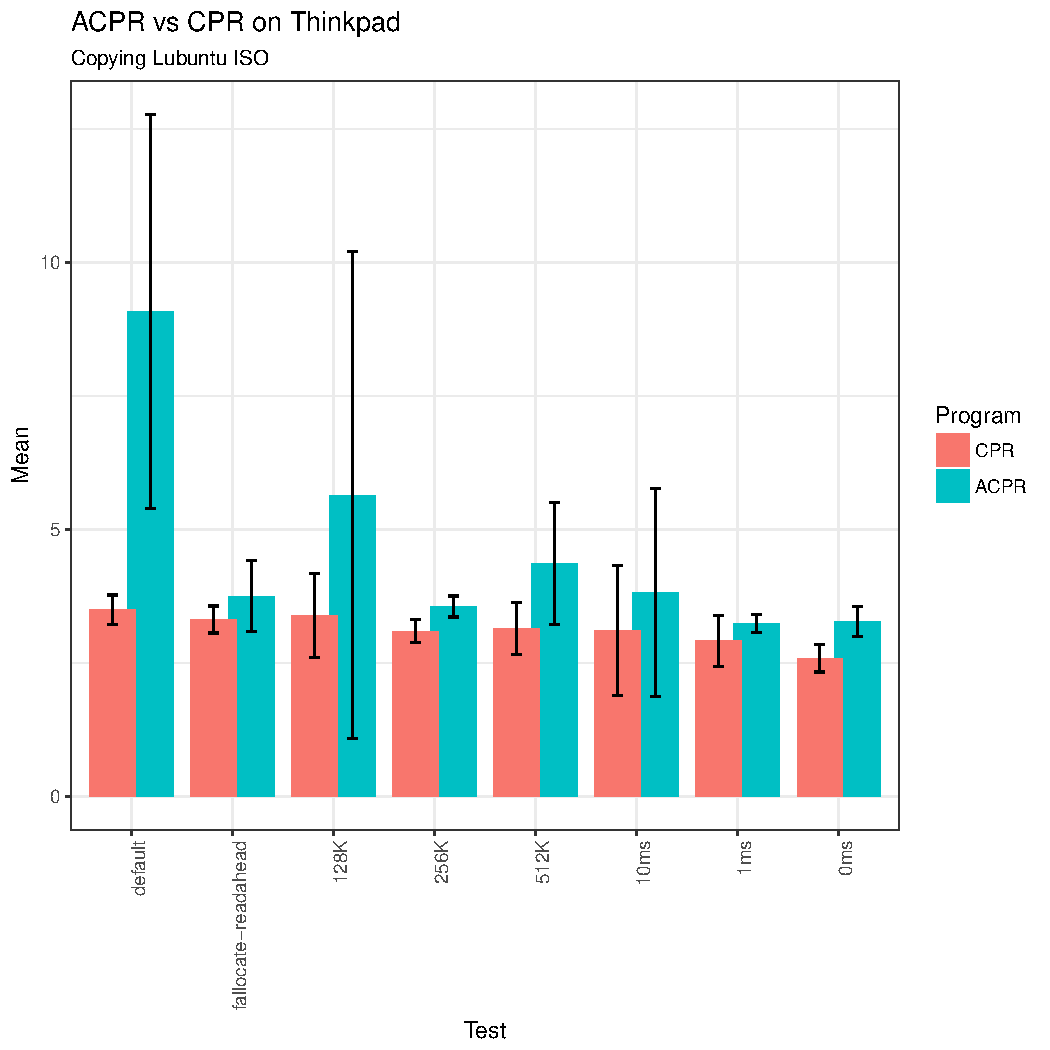
\includegraphics[width=0.8\textwidth,height=0.8\textheight,]{Laptop_Lubuntu_Barplot.pdf}
\end{frame}

\begin{frame}
\frametitle{Evaluation: SSD}
\begin{enumerate}[1.]
	\item{Copying Linux Source}
	\begin{itemize}
		\item Both \texttt{cp} and \texttt{acpr} quite slow: 12.75s and 15.05s by default
		\item Tried raising threshold for using AIO (since most files small), slight performance boost to 13.69s
		\item Tried smaller block size (since most files small), slight performance boost to 14.37s
		\item Tried increasing number of \texttt{iocb} used per file copy, performance loss
		\item Again, adjusting timeout had negligible effect
	\end{itemize}
\end{enumerate}
\end{frame}

\begin{frame}
    \frametitle{Evaluation: SSD}
    \framesubtitle{Copying Linux 4.4 on Laptop}
    \centering
    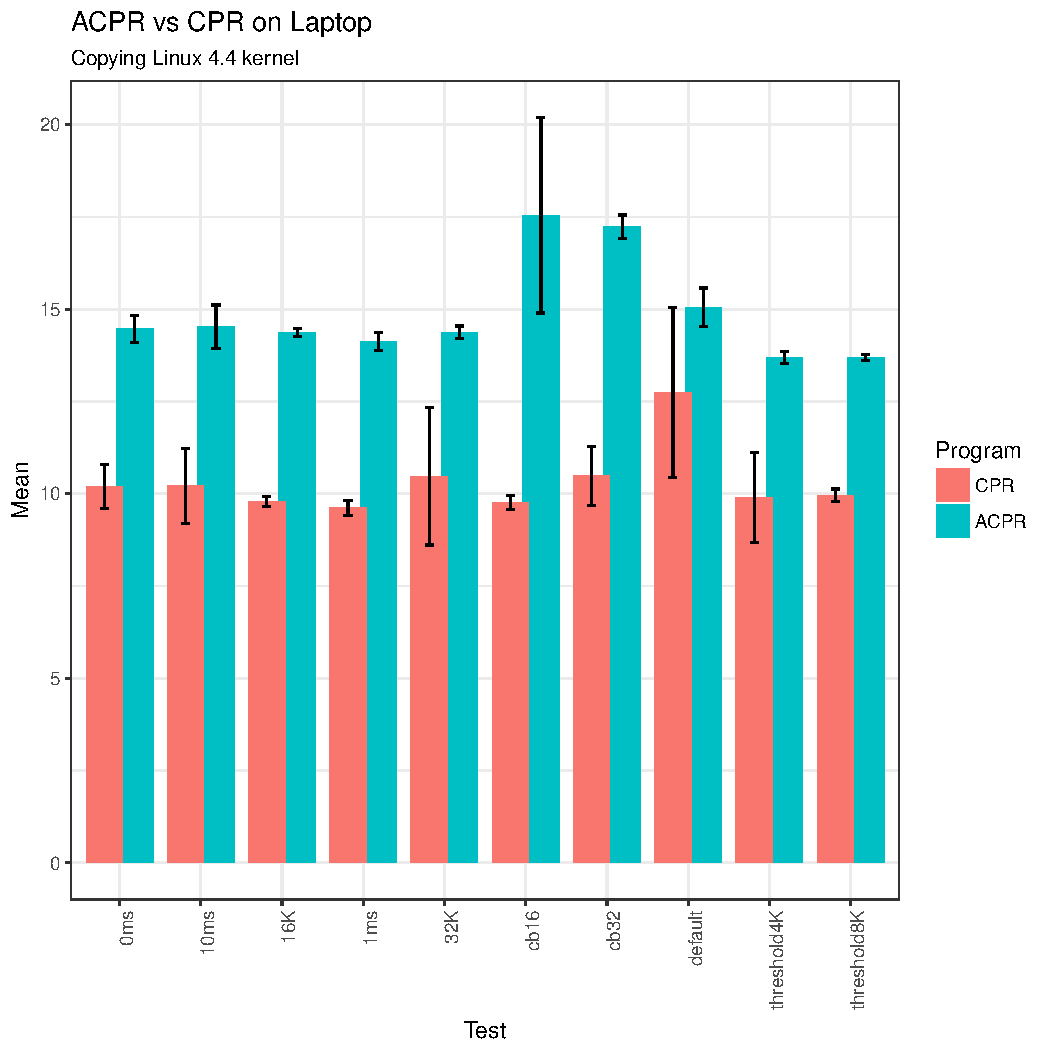
\includegraphics[width=0.8\textwidth,height=0.8\textheight,]{Laptop_Linux_Barplot.pdf}
\end{frame}

\begin{frame}
\frametitle{Evaluation: HDD}
\begin{enumerate}[1.]
	\item{Environment}
	\begin{itemize}
		\item zerberus.csres.utexas.edu
		\item 32-core Xeon system, 128 GB RAM, 7200 RPM Hard Disk
	\end{itemize}
	\item{Copying Large Files}
	\begin{itemize}
		\item \texttt{cp} took 5.82s, \texttt{acpr} 5.86s
		\item Increasing block size slowed it down
		\item For all other experiments, negligible changes
		\item We attribute this to disk bottleneck as we are flushing before each iteration
	\end{itemize}
	\item{Copying Linux Source}
	\begin{itemize}
		\item Slow for both: \texttt{cp} took 14.9s, \texttt{acpr} 34.6s
		\item For all other experiments, negligible changes as well
	\end{itemize}
\end{enumerate}
\end{frame}

\begin{frame}
    \frametitle{Evaluation: HDD}
    \framesubtitle{Copying Lubuntu ISO}
    \centering
    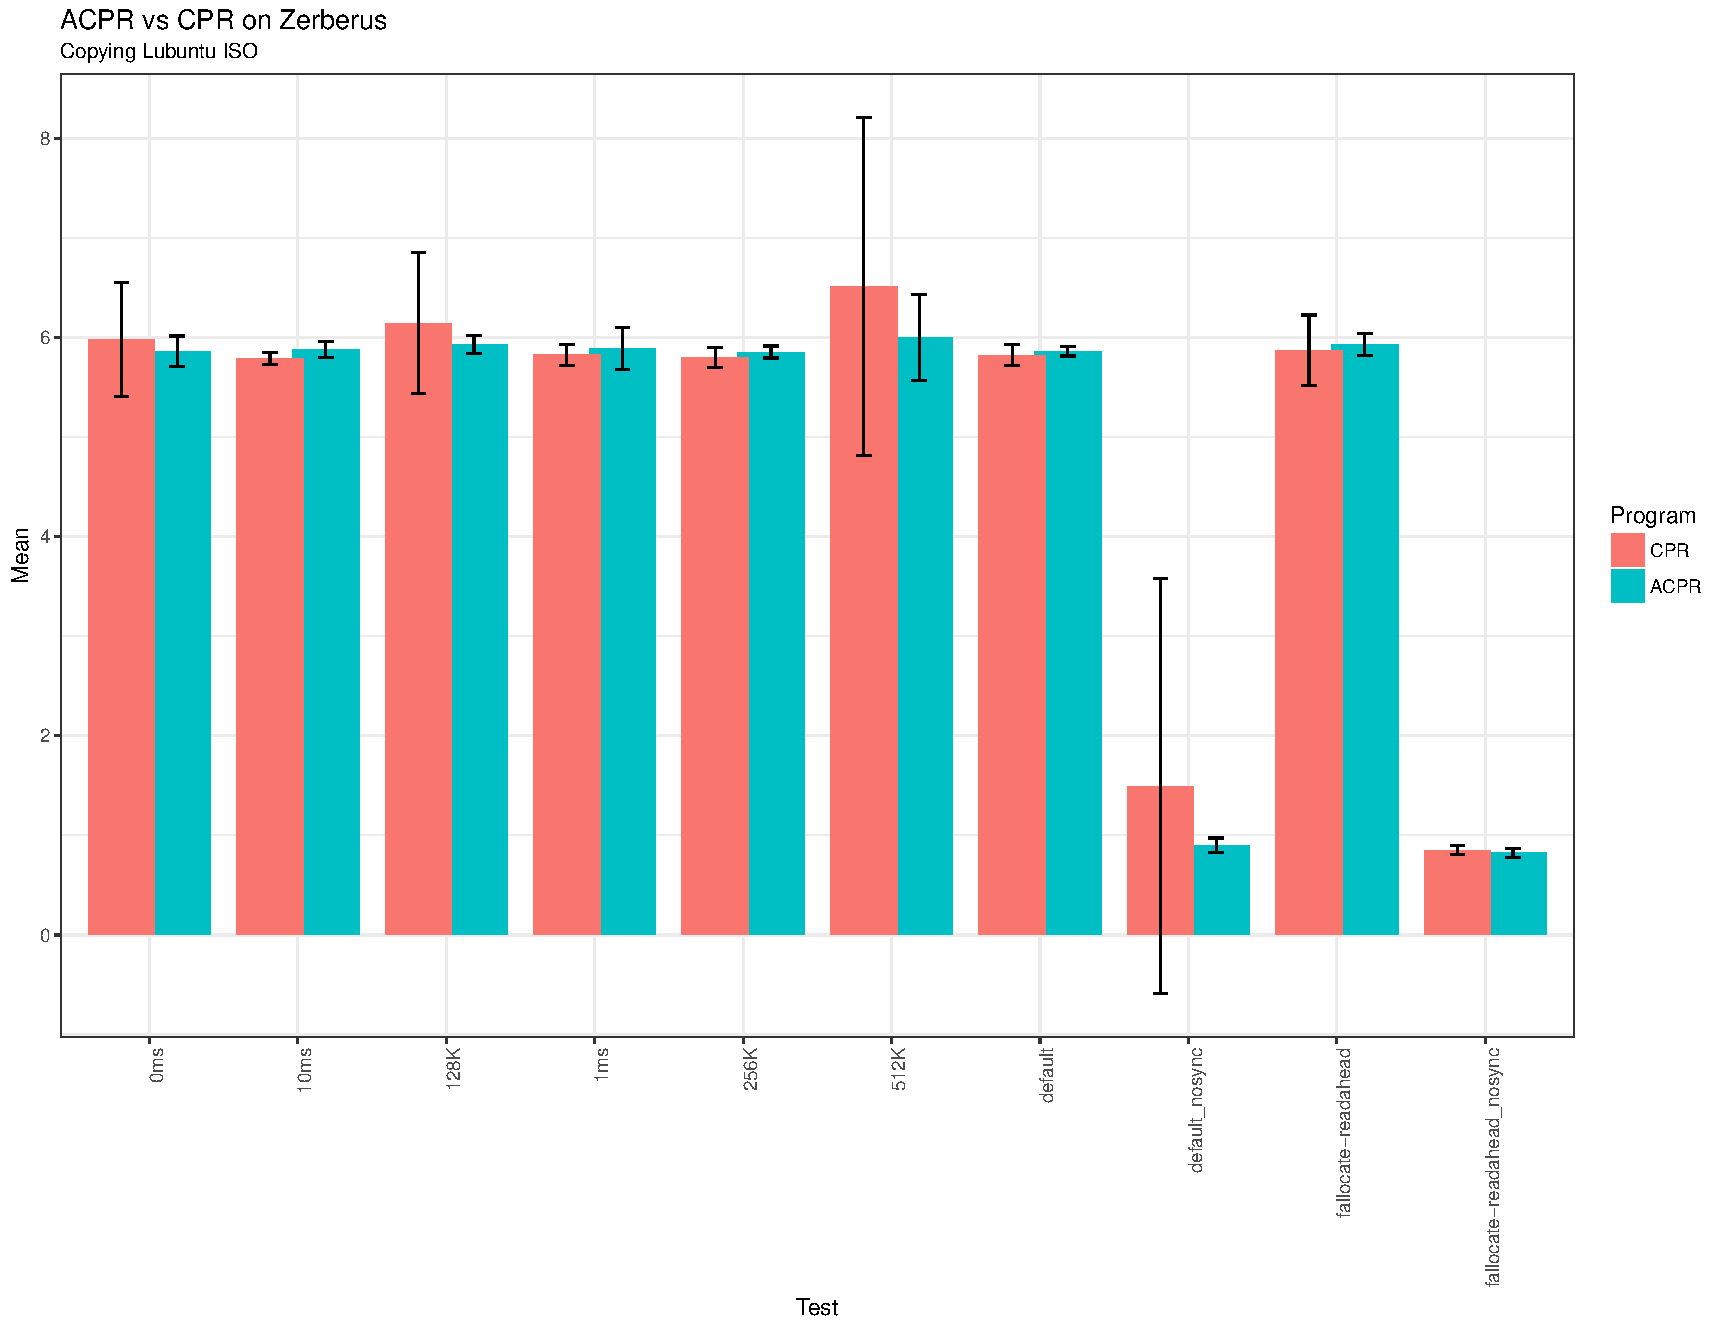
\includegraphics[width=0.8\textwidth,height=0.8\textheight,]{CSRES_Lubuntu_Barplot.pdf}
\end{frame}

\begin{frame}
    \frametitle{Evaluation: HDD}
    \framesubtitle{Copying Linux 4.4 on Laptop}
    \centering
    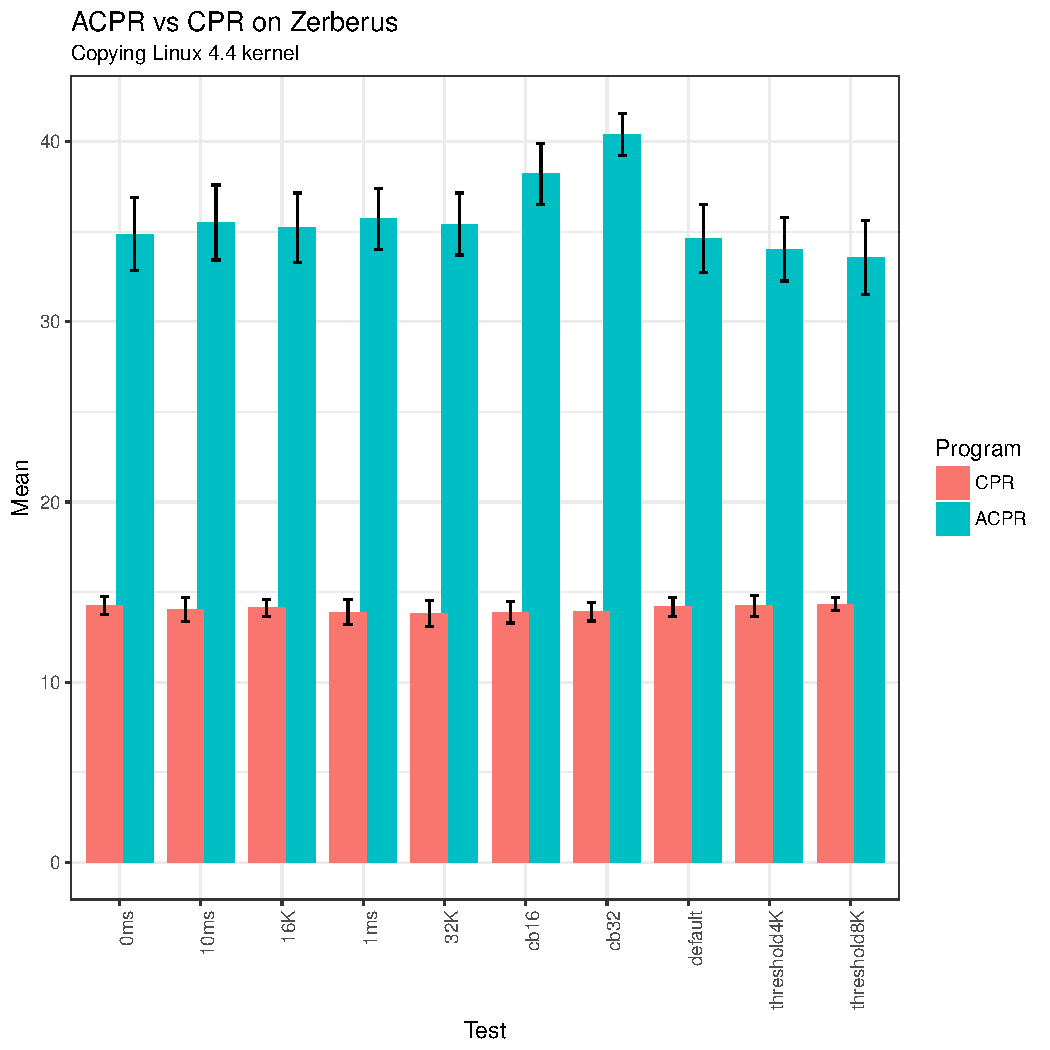
\includegraphics[width=0.8\textwidth,height=0.8\textheight,]{CSRES_Linux_Barplot.pdf}
\end{frame}

\begin{frame}
\frametitle{Evaluation: HDD}
\begin{enumerate}[1.]
\item{Copying Large Files, Without Caching}
\begin{itemize}
	\item If disk is the bottleneck, what if we disable flushing before each test?
	\item As expected, giant performance jump: \texttt{cp} 1.49s, \texttt{acpr} 0.9s
	\item Using fallocate and readahead and re-running yields more improvmeent: \texttt{cp} 0.85s, \texttt{acpr} 0.82s
	\item We beat cp!
	\item Possibly due to the kernel using different memory management strategies? Not fully certain what the cause is since both should be served from buffer cache.
\end{itemize}
\end{enumerate}
\end{frame}

\section{Conclusion}
\begin{frame}
\frametitle{Conclusion}
\begin{enumerate}[1.]
\item Got close (or surpassed in two cases) \texttt{cp} performance using AIO
\item Effects were more pronounced on SSD than HDD, since HDD was heavy bottleneck
\item Improvements: multi-threaded event processing, support symlinks, batching write task submissions
\end{enumerate}
\end{frame}

\begin{frame}
    \frametitle{References}
    \footnotesize{
        \begin{thebibliography}{99}
            \bibitem{aio7}
                aio(7), http://man7.org/linux/man-pages/man7/aio.7.html
            \bibitem{ubuntu}
            	Asynchronous IO, http://manpages.ubuntu.com/manpages/precise/en/man3/io.3.html
        \end{thebibliography}
        }
\end{frame}

\end{document}
